% !TeX spellcheck = en_GB
\documentclass{article}

\usepackage{float}
\usepackage[hidelinks]{hyperref}
\usepackage{graphicx}
\usepackage{caption}
\usepackage{tabu}
\usepackage{subcaption}
\usepackage{adjustbox}
\usepackage[utf8]{inputenc}
\usepackage[colorinlistoftodos,]{todonotes}
\usepackage{cite}
\usepackage[nottoc,numbib]{tocbibind}

\newcommand{\newpar}{\bigskip\noindent}
\bibliographystyle{plain}
\presetkeys{todonotes}{inline}{}

\author{Anders Wind Steffensen (awis@itu.dk)\and Mikael Lindemann (mlin@itu.dk)\\\\Supervisor: Sebastian Risi (sebr@itu.dk)}
\title{Shortest Path in Undirected Unweighted Graphs using Evolvable Neural Turing Machine}

\begin{document}
\maketitle
\tableofcontents
\listoftodos
\newpage
\section{Introduction}
Finding the shortest path in a graph is one of the most well studied algorithmic graph problems and solutions for the problem origin back to the late 1950's.\todo[color=green]{maybe ref?} Finding the shortest path has a long list of applications from transport and routing tables in networks to being an essential part of many more advanced graph algorithms. Most problems can be modelled as a shortest path problem on a large enough graph and as such it can be seen as a general problem solver.\todo[color=green]{check liiiige om det her er bullshit - eller find en reference.} In recent years neural networks has gained more and more traction in the artificial intelligence and machine learning fields. This change is both due to the more widespread adoption and advancement of graphical processing units but also due to theoretical breakthroughs.\todo[color=green]{ref?} Neural networks are used for classification, finding heuristics and as the decision mechanism for artificial agents among others.

\newpar One of the most often mentioned problems with neural networks and machine learning in general is that they are inherently single purpose and do not handle different problems and domains very well from what they are trained to do.\todo[color=green]{skal her refereres til den artikel som Sebastian sendte omkring planning problems?}

\newpar With the introduction of neural networks with memory more domains should be feasibly solvable. In \todo[color=green]{X article} a neural differentiable computer was shown to be able to find the shortest path in the London underground by using memory to store variables and information about the graph.

\newpar In this report we want to examine how well these neural networks with memory can handle the shortest path problem on undirected, unweigthed general graphs.\todo{Genskriv dette når vi har lavet forsøgene, så vi ikke lover mere end vi kan holde.}

\section{Background}
\subsection{Graphs}
A \textit{graph} $G(V,E)$ is data-structure which consists of a set of \textit{vertices} $V$ and a set of \textit{edges} $E$ where an edge is a pair of vertices $(u,v)$. An \textit{undirected graph} implies that if edge $ (u,v) $ exists then $ (v,u) $ exists in the graph. An \textit{unweighted graph} every edge is equal in the cost to traverse it.
Two vertices are \textit{adjacent} if they are part of the same edge $ e $. A \textit{path} $ P $ is a ordered set of edges such that every consecutive edge shares a vertex. To vertices $ u $, $ v $ are \textit{connected} if there exist a path between $ u $, $ v $.

\newpar In an undirected unweighted graph the length of a path P is $ |P| $. A shortest path between two vertices  $ u $, $ v $ is a path $ P $ connecting  $ u $, $ v $ of the smallest length. The Breadth First Search (BFS) algorithm can find the shortest path in time $ \mathcal{O}(n+m) $ where $ n=|V| $ and $ m=|E| $. To be able to solve this combinatorial problem for which the exhaustive search space is $ n! $ the BFS algorithm uses a queue to store previously visited vertices and a map of the vertices and which vertex would come before it in the shortest path.

\todo{why is memory neccesary or maybe further in}

\subsection{Neural Networks}
A \textit{neural network} is an approximation method for \textit{n} dimensional functions. Neural networks consists of a collection of \textit{layers} $L_1 .. L_n$ where $L_1$ is the \textit{input layer}, $L_2 .. L_{n-1}$ are \textit{hidden layers}, and $L_n$ is the \textit{output layer}. Each layer $ Li $ consist of a number of \textit{neurons}. A neuron is connected to other neurons in the layer before and after its own layer.\todo{skal vi nævne at man også kan forbindes til sig selv?} Neurons can send signals to other neurons it is connected to. The strength of a signal is specified by a \textit{signal function} of a neuron. Neurons gets \textit{activated} and sends a signal if itself has become activated a \textit{threshold} amount by other neurons. The signal function is based on a \textit{formula}, a \textit{weight} and a \textit{bias}. 

\newpar The \textit{feed forward algorithm} activates the neurons of the input layer based on some input data, whom in return activates the neurons of the next layer and so on. The values of the output layer is then read. The \textit{backpropagation algorithm} calculates the error of the output neurons compared to the input data and corrects it based on a function. The errors are then backpropagated through the layers. By running the feed forward and backpropagation algorithms in combination with enough data, almost any function can be approximated.

\newpar A \textit{one hot encoding} of a nominal data point, is a conversion of the data point into a bit array $A$ with the length $n$, where $n$ is the number of possible nominal values. Each of the nominal values are then assigned a label $i \in \{0 .. n-1\}$. For a nominal value with label $i$ only $ A[i] $ is $1$. All other elements in $A$ is $0$.

\subsection{Evolutionary Neural Networks}
Evolutionary neural networks is a method of training and developing the topology of neural networks based on evolutionary algorithms. These networks can be trained without using supervised learning but reward based learning where a fitness function describes how well the network does in the specific instance. 

\subsubsection{NeuroEvolution of Augmenting Topologies (NEAT)}
Whereas most other Evolutionary Neural Network algorithms, start from a randomly seeded network, NEAT evolves the topology from the minimal network, where no hidden neurons exist.

\newpar NEAT also uses a technique called innovation numbering, in order to distinguish or compare genes between phenomes. The technique is used both when mating, that is, pairing two phenomes in order to produce new outspring, and when "clustering" the phenomes into species.

\newpar The notion of species is used to protect innovative but untrained structures in a phenome. The idea is that, when a new structure has been evolved, it might not have good weights associated, which means that it will initially perform much worse than older and trained phenomes without this structure. Instead of making all phenomes compete against each other, the phenomes are divided into species, that can then compete against each other. This allows the innovative mutations to last a few generations, so they can prove (or disprove) their worth.

\newpar Further details about the NEAT algorithm can be found in \cite{stanley2002evolving}.

\subsection{Evolvable Neural Turing Machine}
In \todo{cite entm} Greve et. al. introduces the Evolvable Neural Turing Machine. A Neural Turing Machine is able to write and read of a non-fixed size memory bank like a regular turing machine. Greve et. al. shows that the evolvable neural turing machine are able to solve simple algorithm tasks such as the copy task, and the continuous T-maze task.

\section{Experiment}
Given an unweighted undirected graph $G$, a source vertex $s$, and a target vertex $t$, find the shortest path from $s$ to $t$ in $G$.

\newpar We have restricted the problem to instances where a path between $s$ and $t$ exists.

\subsection{Instance encoding}
In order to feed the instance into the network, we use a one hot encoding of the adjacency matrix of the graph and each of the source and target vertices. See \autoref{fig:input:encoding} for an example.

\begin{figure}[ht]
	\centering
	\begin{subfigure}{.5\textwidth}
		\centering
		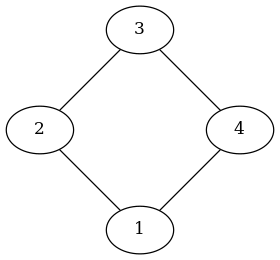
\includegraphics[width=\textwidth]{figures/encoding.png}
		\subcaption{}
	\end{subfigure}%
	\begin{subfigure}{.5\textwidth}
		\centering
		\begin{tabular}{|c|c|c|c|c|}
			\hline
			&\textbf{1}&\textbf{2}&\textbf{3}&\textbf{4}\\\hline
			\textbf{1}&0&1&0&0\\\hline
			\textbf{2}&1&0&1&1\\\hline
			\textbf{3}&0&1&0&1\\\hline
			\textbf{4}&0&1&1&0\\\hline
		\end{tabular}
		\subcaption{}
	\end{subfigure}\par\bigskip
	\begin{adjustbox}{center}
		\begin{subfigure}{1.3\textwidth}
			\centering
			\begin{tabu}{|c|c|c|c||c|c|c|c||c|c|c|c||c|c|c|c|[2pt]c|c|c|c|[2pt]c|c|c|c|}
				\hline
				0&1&0&0&1&0&1&1&0&1&0&1&0&1&1&0&1&0&0&0&0&0&0&1\\\hline
			\end{tabu}
			\subcaption{}
		\end{subfigure}
	\end{adjustbox}
	\caption{Shows a simple graph (a), its adjancency matrix (b) and an encoding where $s=1$ and $t=4$ (c). Thick lines between cells means encoding of a new structure. The three structures are the flattened adjacency table, with each row delimited with double lines for visibility, the one-hot encoding of $s$, and the one-hot encoding of $t$}
	\label{fig:input:encoding}
\end{figure}

\noindent When the neural network using the turing machine returns output, this is a one-hot encoding of the next vertex on the path to the target. Furthermore, for simplicity we choose the first node with maximal weight.

\newpar This means that we can run the graph through the neural network multiple times, and each time, the neural network will tell us which vertex to move to, which we can give it back as the new source vertex to move from.

\subsection{Instance generation}
Each experiment has a few settings that can be chosen between.
A number of these settings are related to instance generation.

\newpar We have made a factory that produces graphs containing a path of a specified length, but with the rest of the vertices connected to this path, in some fashion.

\newpar The configurations that can be chosen between for this factory is the following:

\begin{itemize}
	\item The number of vertices of the graph
	\item The length of the path that should be found in the graph
	\item The seed of the random number generator that is used to produce instances
	\item Whether or not the same graph should be used in symmetric instances, that is, one instance with a source and goal and another where they have been switched.
\end{itemize}

\noindent The factory then chooses a source and a goal, and builds a path of the specified length between them.
If there are any unused vertices left in the graph, they will become adjacent to some other vertex in the connected component of the path.
The last part is implemented to try to confuse the neural networks, since the input is given to them as an adjacency matrix.

\subsection{Fitness}
We have chosen to give the following scores for the output of each step on the shortest path:

\begin{itemize}
	\item[1] if there is an edge from the current vertex to the chosen vertex, but the distance from the chosen vertex to the goal vertex is greater than from the current vertex to the goal vertex.
	\item[2] if there is an edge from the current vertex to the chosen vertex, but the distance from the chosen vertex to the goal vertex is the same as from the current vertex to the goal vertex.
	\item[4] if there is an edge from the current vertex to the chosen vertex, but the distance from the chosen vertex to the goal vertex is less than from the current vertex to the goal vertex.
\end{itemize}

\noindent Furthermore, we give the score 0, if one step resulted in a move where no edge exists. Also the accumulated score is reset to 0, and no further steps are performed.

\newpar The idea behind these scores is that we want to reward neural networks that understand the underlying graph problem (or can at least guess them) more than a network that chooses arbitrarily.

\subsection{The Experiments}
To assess and measure how well the shortest path problem is solved, two times three experiments are performed. The first three experiments uses the NEAT framework to train and build the neural networks. The last three experiments uses the ENTM extension of the NEAT framework and can therefore in addition approximate Neural Turing machines. The memory is unlimited (within the bounds of the host machine), the write vector size is 4 and the default jump mechanism introduced in \cite{greve2016evolving} is used. 

\newpar Both networks uses the exact same configuration for NEAT and the general problem to make it easier to compare the two. Each configuration uses 30 species with population of 500. Each genome is tested on 25 unique graphs per generation. The entire configuration can be seen in appendix \todo{appendix}. 

\section{Results}
The results of the experiments can be seen on figure \ref{experiments:graph:1}. The $ y $ axis shows the fitness of the champion whereas the $ x $ axis shows the generation. The experiments shown with blue represents the configuration without memory and those shown in red with memory. 

\begin{figure}[ht]
	\todo[inline]{TODO}
	\caption{Graph of the results}
	\label{experiments:graph:1}
\end{figure}



\section{Analysis}



\section{Conclusion}

\newpage
\bibliography{bibliography}

\newpage

\appendix
\section{SharpNEAT Configuration File}
\end{document}
